%
% grundlagen.tex -- Grundlagen
%
% (c) 2021 Prof Dr Andreas Müller, OST Ostschweizer Fachhochschule
%
\section{Grundlagen
\label{buch:section:grundlagen}}
\rhead{Grundlagen}
Die Potenzen $A^k$ sind besonders einfach zu berechnen, wenn die Matrix
Diagonalform hat, wenn also $A=\operatorname{diag}(\lambda_1,\dots,\lambda_n)$
ist.
In diesem Fall ist $Ae_k=\lambda_k e_k$ für jeden Standardbasisvektor $e_k$.
Statt sich auf Diagonalmatrizen zu beschränken könnten man also auch
Vektoren $v$ suchen, für die gilt $Av=\lambda v$, die also von $A$ nur
gestreckt werden.
Gelingt es, eine Basis aus solchen sogenanten {\em Eigenvektoren} zu finden,
dann kann man die Matrix $A$ durch Basiswechsel in diese Form bringen.

\begin{figure}
\centering
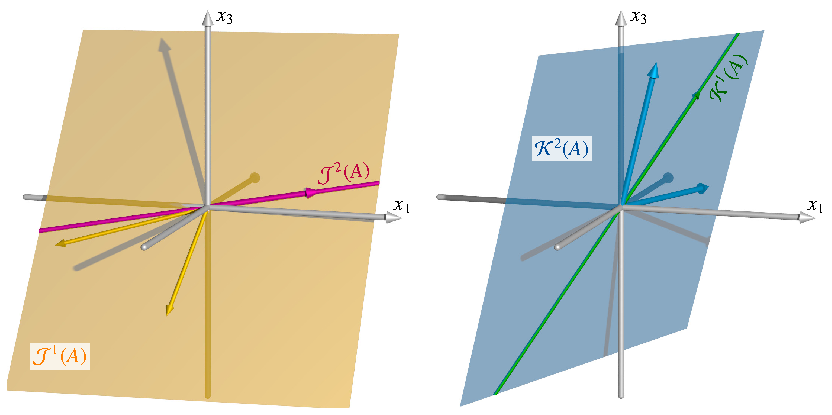
\includegraphics[width=\textwidth]{chapters/40-eigenwerte/images/kernbild.pdf}
\caption{Iterierte Kerne und Bilder einer $3\times 3$-Matrix mit Rang~2.
Die abnehmend geschachtelten iterierten Bilder
$\mathcal{J}^1(A) \subset \mathcal{J}^2(A)$
sind links dargestellt, die zunehmen geschachtelten iterierten Kerne
$\mathcal{K}^1(A) \subset \mathcal{K}^2(A)$ rechts.
\label{buch:eigenwerte:img:kernbild}}
\end{figure}

\begin{figure}
\centering
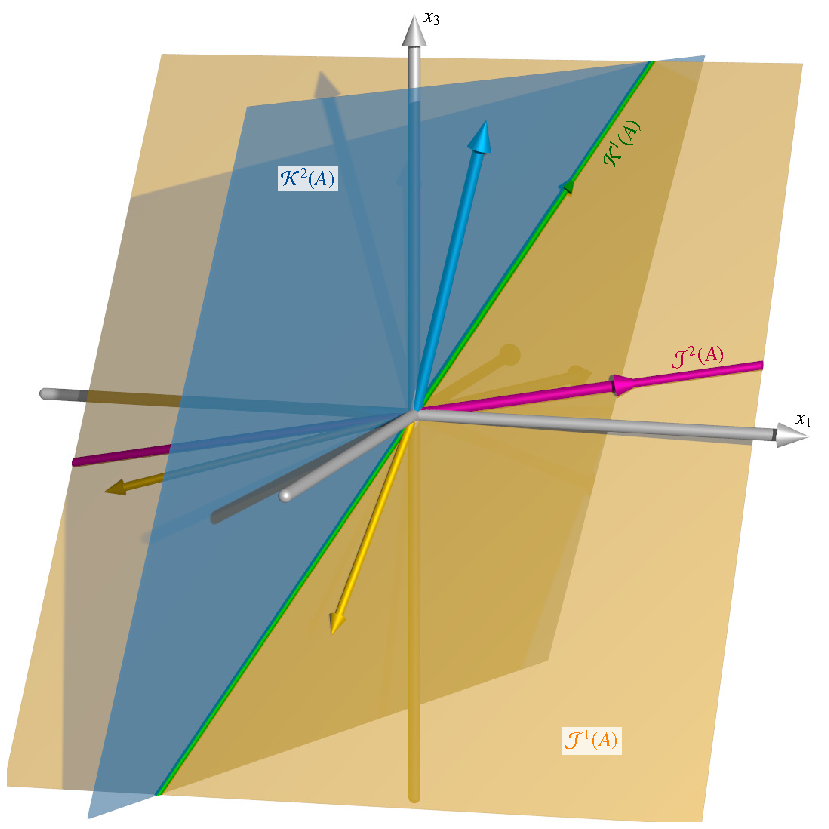
\includegraphics[width=\textwidth]{chapters/40-eigenwerte/images/kombiniert.pdf}
\caption{Iterierte Kerne und Bilder einer $3\times 3$-Matrix mit Rang~2.
Da $\dim\mathcal{J}^2(A)=1$ und $\dim\mathcal{J}^1(A)=2$ ist, muss es
einen Vektor in $\mathcal{J}^1(A)$ geben, der von $A$ auf $0$ abgebildet
wird, der also auch im Kern $\mathcal{K}^1(A)$ liegt.
Daher ist $\mathcal{K}^1(A)$ die Schnittgerade von $\mathcal{J}^1(A)$ und
$\mathcal{K}^2(A)$.
Man kann auch gut erkennen, dass
$\mathbb{R}^3
=
\mathcal{K}^1(A)\oplus \mathcal{J}^1(A)
=
\mathcal{K}^2(A) \oplus \mathcal{J}^2(A)$
ist.
\label{buch:eigenwerte:img:kombiniert}}
\end{figure}

%
% Kern und Bild von Matrixpotenzen
%
\subsection{Kern und Bild von Matrixpotenzen
\label{buch:subsection:kern-und-bild}}
In diesem Abschnitt ist $A\in M_n(\Bbbk)$, $A$ beschreibt eine lineare
Abbildung $f\colon\Bbbk^n\to \Bbbk^n$.
In diesem Abschnitt sollen Kern und Bild der Potenzen $A^k$ untersucht
werden.
\begin{definition}
Wir bezeichnen Kern und Bild der iterierten Abbildung $A^k$ mit
\[
\mathcal{K}^k(A)
=
\ker A^k
\qquad\text{und}\qquad
\mathcal{J}^k(A)
=
\operatorname{im} A^k.
\]
\end{definition}

Durch Iteration wird das Bild immer kleiner.
Wegen
\[
\mathcal{J}^k (A)
=
\operatorname{im} A^k
=
\operatorname{im} A^{k-1} A
=
\{ A^{k-1} Av\;|\; v \in \Bbbk^n\}
\subset
\{ A^{k-1} v\;|\; v \in \Bbbk^n\}
=
\mathcal{J}^{k-1}(A)
\]
folgt
\begin{equation}
\Bbbk^n
=
\operatorname{im}E
=
\operatorname{im}A^0
=
\mathcal{J}^0(A)
\supset
\mathcal{J}^1(A)
=
\operatorname{im}A
\supset
\mathcal{J}^2(A)
\supset\dots\supset
\mathcal{J}^k(A)
\supset
\mathcal{J}^{k+1}(A)
\supset \dots \supset
\{0\}.
\label{buch:eigenwerte:eqn:Jkchain}
\end{equation}
Für die Kerne gilt etwas Ähnliches.
Ein Vektor $x\in \mathcal{K}^k(A)$ erfüllt $A^kx=0$.
Dann erfüllt er aber erst recht auch
\[
A^{k+1}x=A\underbrace{A^kx}_{\displaystyle=0}=0,
\]
also ist $x\in\mathcal{K}^k(A)$.
Es folgt
\begin{equation}
\{0\}
=
\mathcal{K}^0(A) = \ker A^0 = \ker E
\subset
\mathcal{K}^1(A) = \ker A
\subset
\dots
\subset
\mathcal{K}^k(A)
\subset
\mathcal{K}^{k+1}(A)
\subset
\dots
\subset
\Bbbk^n.
\label{buch:eigenwerte:eqn:Kkchain}
\end{equation}
Neben diesen offensichtlichen Resultaten kann man aber noch mehr
sagen.
Es ist klar, dass in beiden Ketten
\label{buch:eigenwerte:eqn:Jkchain}
und
\label{buch:eigenwerte:eqn:Kkchain}
nur in höchstens $n$ Schritten eine wirkliche Änderung stattfinden 
kann.
Man kann aber sogar genau sagen, wo Änderungen stattfinden:

\begin{satz}
\label{buch:eigenwerte:satz:ketten}
Ist $A\in M_n(\Bbbk)$ eine $n\times n$-Matrix, dann gibt es eine Zahl $k$
so, dass
\[
\begin{array}{rcccccccccccl}
0=\mathcal{K}^0(A)
&\subsetneq& \mathcal{K}^1(A) &\subsetneq& \mathcal{K}^2(A)
&\subsetneq&\dots&\subsetneq&
\mathcal{K}^k(A) &=& \mathcal{K}^{k+1}(A) &=& \dots
\\
\Bbbk^n= \mathcal{J}^0(A)
&\supsetneq& \mathcal{J}^1(A) &\supsetneq& \mathcal{J}^2(A)
&\supsetneq&\dots&\supsetneq&
\mathcal{J}^k(A) &=& \mathcal{J}^{k+1}(A) &=& \dots
\end{array}
\]
ist.
\end{satz}

\begin{proof}[Beweis]
Es sind zwei Aussagen zu beweisen.
Erstens müssen wir zeigen, dass die Dimension von $\mathcal{K}^i(A)$ 
nicht mehr grösser werden kann, wenn sie zweimal hintereinander gleich war.
Nehmen wir daher an, dass $\mathcal{K}^i(A) = \mathcal{K}^{i+1}(A)$.
Wir müssen $\mathcal{K}^{i+2}(A)$ bestimmen.
$\mathcal{K}^{i+2}(A)$ besteht aus allen Vektoren $x\in\Bbbk^n$ derart,
dass $Ax\in \mathcal{K}^{i+1}(A)=\mathcal{K}^i(A)$ ist.
Daraus ergibt sich, dass $AA^ix=0$, also ist $x\in\mathcal{K}^{i+1}(A)$.
Wir erhalten also
$\mathcal{K}^{i+2}(A)\subset\mathcal{K}^{i+1}\subset\mathcal{K}^{i+2}(A)$,
dies ist nur möglich, wenn beide gleich sind.

Analog kann man für die Bilder vorgehen.
Wir nehmen an, dass $\mathcal{J}^i(A) = \mathcal{J}^{i+1}(A)$ und
bestimmten $\mathcal{J}^{i+2}(A)$.
$\mathcal{J}^{i+2}(A)$ besteht aus all jenen Vektoren, die als
$Ax$ mit $x\in\mathcal{J}^{i+1}(A)=\mathcal{J}^i(A)$ erhalten
werden können.
Es gibt also insbesondere ein $y\in\Bbbk^i$ mit $x=A^iy$.
Dann ist $Ax=A^{i+1}y\in\mathcal{J}^{i+1}(A)$.
Insbesondere besteht $\mathcal{J}^{i+2}(A)$ genau aus den Vektoren
von $\mathcal{J}^{i+1}(A)$.

Zweitens müssen wir zeigen, dass die beiden Ketten bei der gleichen
Potenz von $A$ konstant werden.
Dies folgt jedoch daraus, dass $\dim\mathcal{J}^i(A) = \operatorname{Rang} A^i
= n - \dim\ker A^i = n -\dim\mathcal{K}^i(A)$.
Der Raum $\mathcal{J}^k(A)$ hört also beim gleichen $i$ auf, kleiner
zu werden, bei dem auch $\mathcal{K}^i(A)$ aufhört, grösser zu werden.
\end{proof}

\begin{satz}
Die Zahl $k$ in Satz~\ref{buch:eigenwerte:satz:ketten}
ist nicht grösser als $n$, also
\[
\mathcal{K}^n(A) = \mathcal{K}^l(A)
\qquad\text{und}\qquad
\mathcal{J}^n(A) = \mathcal{J}^l(A)
\]
für $l\ge n$.
\end{satz}

\begin{proof}[Beweis]
Nach Satz~\ref{buch:eigenwerte:satz:ketten} muss die
Dimension von $\mathcal{K}^i(A)$ in jedem Schritt um mindestens
$1$ zunehmen, das ist nur möglich, bis zur Dimension $n$.
Somit können sich $\mathcal{K}^i(A)$ und $\mathcal{J}^i(A)$ für $i>n$
nicht mehr ändern.
\end{proof}

\begin{definition}
\label{buch:eigenwerte:def:KundJ}
Die gemäss Satz~\ref{buch:eigenwerte:satz:ketten} identischen Unterräume
$\mathcal{K}^i(A)$ für $i\ge k$ und die identischen Unterräume
$\mathcal{J}^i(A)$ für $i\ge k$ werden mit
\[
\begin{aligned}
\mathcal{K} &= \mathcal{K}^i(A)&&\forall i\ge k \qquad\text{und}
\\
\mathcal{J} &= \mathcal{J}^i(A)&&\forall i\ge k
\end{aligned}
\]
bezeichnet.
\end{definition}

%
% Inveriante Unterräume
%
\subsection{Invariante Unterräume
\label{buch:subsection:invariante-unterraeume}}
Kern und Bild sind der erste Schritt zu einem besseren Verständnis 
einer linearen Abbildung oder ihrer Matrix.
Invariante Räume dienen dazu, eine lineare Abbildung in einfachere
Abbildungen zwischen ``kleineren'' Räumen zu zerlegen, wo sie leichter
analysiert werden können.

\begin{definition}
Sei $f\colon V\to V$ eine lineare Abbildung eines Vektorraums in sich
selbst.
Ein Unterraum $U\subset V$ heisst {\em invarianter Unterraum},
wenn
\[
f(U) = \{ f(x)\;|\; x\in U\} \subset U
\]
gilt.
\end{definition}

Der Kern $\ker A$  einer linearen Abbildung ist trivialerweise ein
invarianter Unterraum, da alle Vektoren in $\ker A$ auf $0\in\ker A$
abgebildet werden.
Ebenso ist natürlich $\operatorname{im}A$ ein invarianter Unterraum,
denn jeder Vektor wird in $\operatorname{im}A$ abgebildet, insbesondere
auch jeder Vektor in $\operatorname{im}A$.

\begin{satz}
\label{buch:eigenwerte:satz:KJinvariant}
Sei $f\colon V\to V$ eine lineare Abbildung mit Matrix $A$.
Jeder der Unterräume $\mathcal{J}^i(A)$ und $\mathcal{K}^i(A)$ 
ist ein invarianter Unterraum.
\end{satz}

\begin{proof}[Beweis]
Sei $x\in\mathcal{K}^i(A)$, es gilt also $A^ix=0$.
Wir müssen überprüfen, dass $Ax\in\mathcal{K}^i(A)$.
Wir berechnen daher $A^i\cdot Ax=A^{i+1}x=A\cdot A^ix = A\cdot 0=0$,
was zeigt, dass $Ax\in\mathcal{K}^i(A)$.

Sei jetzt $x\in\mathcal{J}^i(A)$, es gibt also ein $y\in V$ derart, dass
$A^iy=x$.
Wir müssen überprüfen, dass $Ax\in\mathcal{J}^i(A)$.
Dazu berechnen wir $Ax=AA^iy=A^iAy\in\mathcal{J}^i(A)$, $Ax$ ist also das
Bild von $Ay$ unter $A^i$.
\end{proof}

\begin{korollar}
Die Unterräume $\mathcal{K}(A)\subset V$ und $\mathcal{J}(A)\subset V$
sind invariante Unterräume.
\end{korollar}

Die beiden Unterräume $\mathcal{K}(A)$ und $\mathcal{J}(A)$ sind besonders
interessant, da wir aus der Einschränkung der Abbildung $f$ auf diese
Unterräume mehr über $f$ lernen können.

\begin{satz}
\label{buch:eigenwerte:satz:fJinj}
Die Einschränkung von $f$ auf $\mathcal{J}(A)$ ist injektiv.
\end{satz}

\begin{proof}[Beweis]
Die Einschränkung von $f$ auf $\mathcal{J}^k(A)$ ist
$\mathcal{J}^k(A) \to \mathcal{J}^{k+1}(A)$, nach Definition von
$\mathcal{J}^{k+1}(A)$ ist diese Abbildung surjektiv.
Da aber $\mathcal{J}^k(A)=\mathcal{J}^{k+1}(A)$ ist, ist
$f\colon \mathcal{J}^k(A)\to\mathcal{J}^k(A)$ surjektiv,
also ist $f$ auf $\mathcal{J}^k(A)$ auch injektiv.
\end{proof}

Die beiden Unterräume $\mathcal{J}(A)$ und $\mathcal{K}(A)$
sind Bild und Kern der iterierten Abbildung mit Matrix $A^k$.
Das bedeutet, dass $\dim\mathcal{J}(A)+\mathcal{K}(A)=n$.
Da $\mathcal{K}(A)=\ker A^k$ und andererseits $A$ injektiv ist auf
$\mathcal{J}(A)$, muss $\mathcal{J}(A)\cap\mathcal{K}(A)=0$.
Es folgt, dass $V=\mathcal{J}(A) + \mathcal{K}(A)$.

In $\mathcal{K}(A)$ und $\mathcal{J}(A)$ kann man unabhängig voneinander
jeweils eine Basis wählen.
Die Basen von $\mathcal{K}(A)$ und $\mathcal{J}(A)$ zusammen ergeben
eine Basis von $V$.
Die Matrix $A'$ in dieser Basis wird die Blockform
\[
A'
=
\left(
\begin{array}{ccc|ccc}
&&&&&\\
&A_{\mathcal{K}'}&&&&\\
&&&&&\\
\hline
&&&&&\\
&&&&A_{\mathcal{J}'}&\\
&&&&&\\
\end{array}
\right)
\]
haben, wobei die Matrix $A_\mathcal{J}'$ invertierbar ist.
Die Zerlegung in invariante Unterräume ergibt also eine natürlich
Aufteilung der Matrix $A$ in kleiner Matrizen mit zum Teil bekannten
Eigenschaften.

%
% Spezialfall, nilpotente Matrizen
%
\subsection{Nilpotente Matrizen
\label{buch:subsection:nilpotente-matrizen}}
Die Zerlegung von $V$ in die beiden invarianten Unterräume $\mathcal{J}(A)$
und $\mathcal{K}(A)$ reduziert die lineare Abbildung auf zwei Abbildungen
mit speziellen Eigenschaften.
Es wurde bereits in Satz~\label{buch:eigenwerte:satz:fJinj} gezeigt,
dass die Einschränkung auf $\mathcal{J}(A)$ injektiv ist.
Die Einschränkung auf $\mathcal{K}(A)$ bildet nach Definition alle
Vektoren nach $k$-facher Iteration auf $0$ ab, $A^k\mathcal{K}(A)=0$.
Solche Abbildungen haben eine speziellen Namen.

\begin{definition}
\label{buch:eigenwerte:def:nilpotent}
Eine Matrix $A$ heisst nilpotent, wenn es eine Zahl $k$ gibt, so dass
$A^k=0$.
\end{definition}

\begin{beispiel}
Obere (oder untere) Dreiecksmatrizen mit Nullen auf der Diagonalen
sind nilpotent.
Wir rechnen dies wie folgt nach.
Die Matrix $A$ mit Einträgen $a_{ij}$
\[
A=\begin{pmatrix}
  0   &a_{12}&a_{13}&\dots &a_{1,n-1}&a_{1n}   \\
  0   &  0   &a_{23}&\dots &a_{1,n-1}&a_{2n}   \\
  0   &  0   &  0   &\dots &a_{1,n-1}&a_{3n}   \\
\vdots&\vdots&\vdots&\ddots&\vdots   &\vdots   \\
  0   &  0   &  0   &\dots &  0      &a_{n-1,n}\\
  0   &  0   &  0   &\dots &  0      &  0
\end{pmatrix}
\]
erfüllt $a_{ij}=0$ für $i\ge j$.
Wir zeigen jetzt, dass sich bei der Multiplikation die nicht
verschwinden Elemente bei der Multiplikation noch rechts oben
verschieben.
Dazu multiplizieren wir zwei Matrizen $B$ und $C$ mit
$b_{ij}=0$ für $i+k>j$ und $c_{ij}=0$ für $i+l>j$.
In der folgenden graphischen Darstellung der Matrizen sind die
Bereiche, wo die Matrixelemente verschwinden, weiss.
\begin{center}
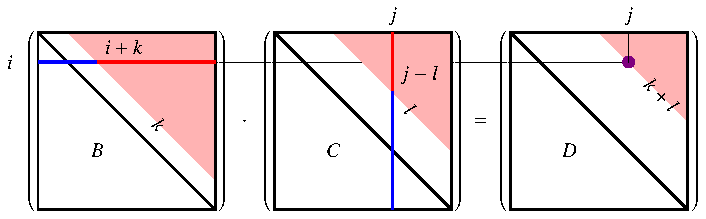
\includegraphics{chapters/40-eigenwerte/images/nilpotent.pdf}
\end{center}
Bei der Berechnung des Elementes $d_{ij}$ wird die Zeile $i$ von $B$
mit der Spalte $j$ von $C$ multipliziert.
Die blau eingefärbten Elemente in dieser Zeile und Spalte sind $0$.
Aus der Darstellung ist abzulesen, dass das Produkt verschwindet, 
die roten, von $0$ verschiedenen Elemente von den blauen Elementen
annihiliert werden.
Dies passiert immer, wenn $i+k>j-l$ ist, oder $i+(k+l)> j$.

Wir wenden diese Beobachtung jetzt auf die Potenzen $A^s$ an.
Für die Matrixelemente von $A^s$ schreiben wir $a^s_{ij}$.
Wir behaupten, dass die Matrixelemente $A^s$ die Bedingung
$a_{ij}^s=0$ für $i+s>j$ erfüllen.
Dies ist für $s=1$ nach Voraussetzung richtig, dies ist die
Induktionsvoraussetzung.
Nehmen wir jetzt an, dass $a_{ij}^s=0$ für $i+s>j$, dann folgt
aus obiger Rechnung, dass $a_{ij}^{s+1}=0$ für $i+s+1>j$, so
dass die Bedingung auch für $A^s$ gilt (Induktionsschritt).
Mit vollständiger Induktion folgt, dass $a_{ij}^s=0$ für $i+s>j$.
Insbesondere ist $A^n=0$, die Matrix $A$ ist nilpotent.
\end{beispiel}

Man kann die Konstruktion der Unterräume $\mathcal{K}^i(A)$ weiter
dazu verwenden, eine Basis zu finden, in der eine nilpotente Matrix
eine besonders einfach Form erhält.

\begin{satz}
\label{buch:eigenwerte:satz:nnilpotent}
Sei $A$ eine nilpotente $n\times n$-Matrix mit der Eigenschaft, dass
$A^{n-1}\ne 0$.
Dann gibt es eine Basis so, dass $A$ die Form
\begin{equation}
A'
=
\begin{pmatrix}
0&1& &      & & \\
 &0&1&      & & \\
 & &0&      & & \\
 & & &\ddots&1& \\
 & & &      &0&1\\
 & & &      & &0\\
\end{pmatrix}
\label{buch:eigenwerte:eqn:nnilpotent}
\end{equation}
bekommt.
\end{satz}

\begin{proof}[Beweis]
Da $A^{n-1}\ne 0$ ist, gibt es einen Vektor $b_n$ derart, dass $A^{n-1}b_n\ne0$.
Wir konstruieren die Vektoren
\[
b_n,\;
b_{n-1}=Ab_n,\;
b_{n-2}=Ab_{n-1},\;
\dots,\;
b_2=Ab_3,\;
b_1=Ab_2.
\]
Aus der Konstruktion folgt $b_1=A^{n-1}b_n\ne 0$, aber $Ab_1=A^nb_n=0$.
Aus der Konstruktion der iterierten Kerne $\mathcal{K}^i(A)$ folgt jetzt,
dass die Vektoren $b_1,\dots,b_n$ eine Basis bilden.
In dieser Basis hat die Matrix die Form~\ref{buch:eigenwerte:eqn:nnilpotent}.
\end{proof}

\begin{definition}
Wir bezeichnen mit $N_n$ eine Matrix der Form
\eqref{buch:eigenwerte:eqn:nnilpotent}.
\end{definition}

Mit etwas mehr Sorgfalt kann man auch die Bedingung, dass $A^{n-1}\ne 0$
sein muss, im Satz~\ref{buch:eigenwerte:satz:nnilpotent} loswerden.

\begin{satz}
\label{buch:eigenwerte:satz:allgnilpotent}
Sei $A$ ein nilpotente Matrix, dann gibt es eine Basis, in der die Matrix
aus lauter Nullen besteht ausser in den Einträgen unmittelbar oberhalb der 
Hauptdiagonalen, wo die Einträge $0$ oder $1$ sind.
Insbesondere zerfällt eine solche Matrix in Blöcke der Form $N_{k_i}$,
$i=1,\dots,l$,
wobei $k_1+\dots+k_l=n$ sein muss:
\begin{equation}
\def\temp#1{\multicolumn{1}{|c}{\raisebox{0pt}[17pt][12pt]{\phantom{x}$#1\mathstrut$}\phantom{x}}}
A'
=\left(
\begin{array}{cccc}
\cline{1-1}
\temp{N_{k_1}} &\multicolumn{1}{|c}{}&        &           \\
\cline{1-2}
          &\temp{N_{k_2}}&\multicolumn{1}{|c}{}&           \\
\cline{2-3}
          &           &\temp{\ddots}&\multicolumn{1}{|c}{}\\
\cline{3-4}
          &           &        &\multicolumn{1}{|c|}{\raisebox{0pt}[17pt][12pt]{\phantom{x}$N_{k_l}$}\phantom{x}}\\
\cline{4-4}
\end{array}
\right)
\label{buch:eigenwerte:eqn:allgnilpotent}
\end{equation}
\end{satz}

Die Einschränkung von $f$ auf den invarianten Unterraum $\mathcal{K}(A)$
ist nilpotent.
Die Zerlegung $V=\mathcal{J}(A)\oplus \mathcal{K}(A)$ führt also zu einer
Zerlegung der Abbildung $f$ in eine invertierbare Abbildung
$\mathcal{J}(A)\to\mathcal{J}(A)$ und eine
nilpotente Abbildung $\mathcal{K}(A)\to\mathcal{K}(A)$.
Nach Satz~\ref{buch:eigenwerte:satz:allgnilpotent} kann man in
$\mathcal{K}(A)$ eine Basis so wählen, dass die Matrix die Blockform
\eqref{buch:eigenwerte:eqn:allgnilpotent} erhält.

%
% Begriff des Eigenwertes und Eigenvektors
%
\subsection{Eigenwerte und Eigenvektoren
\label{buch:subsection:eigenwerte-und-eigenvektoren}}
In diesem Abschnitt betrachten wir Vektorräume $V=\Bbbk^n$ über einem
beliebigen Körper $\Bbbk$ und quadratische Matrizen
$A\in M_n(\Bbbk)$.
In den meisten Anwendungen wird $\Bbbk=\mathbb{R}$ sein.
Da aber in $\mathbb{R}$ nicht alle algebraischen Gleichungen lösbar sind,
ist es manchmal notwendig, den Vektorraum zu erweitern um zum Beispiel
Eigenschaften der Matrix $A$ abzuleiten.

\begin{definition}
Ein Vektor $v\in V$ heisst {\em Eigenvektor} von $A$ zum Eigenwert
$\lambda\in\Bbbk$, wenn $v\ne 0$ und $Av=\lambda v$ gilt.
\end{definition}

Die Bedingung $v\ne 0$ dient dazu, pathologische Situationen auszuschliessen.
Für den Nullvektor gilt $A0=\lambda 0$ für jeden beliebigen Wert von
$\lambda\in\Bbbk$.
Würde man $v=0$ zulassen, wäre jede Zahl in $\Bbbk$ ein Eigenwert,
ein Eigenwert von $A$ wäre nichts besonderes.
Ausserdem wäre $0$ ein Eigenvektor zu jedem beliebigen Eigenwert.

Eigenvektoren sind nicht eindeutig bestimmt, jedes von $0$ verschiedene
Vielfache von $v$ ist ebenfalls ein Eigenvektor.
Zu einem Eigenwert kann man also einen Eigenvektor jeweils mit 
geeigneten Eigenschaften finden, zum Beispiel kann man für $\Bbbk = \mathbb{R}$
Eigenvektoren auf Länge $1$ normieren.
Im Folgenden werden wir oft die abkürzend linear unabhängige Eigenvektoren
einfach als ``verschiedene'' Eigenvektoren bezeichnen.

Wenn $v$ ein Eigenvektor von $A$ zum Eigenwert $\lambda$ ist, dann kann
man ihn mit zusätzlichen Vektoren $v_2,\dots,v_n$ zu einer Basis
$\mathcal{B}=\{v,v_2,\dots,v_n\}$
von $V$ ergänzen.
Die Vektoren $v_k$ mit $k=2,\dots,n$ werden von $A$ natürlich auch
in den Vektorraum $V$ abgebildet, können also als Linearkombinationen
\[
Av = a_{1k}v + a_{2k}v_2 + a_{3k}v_3 + \dots a_{nk}v_n
\]
dargestellt werden.
In der Basis $\mathcal{B}$ bekommt die Matrix $A$ daher die Form
\[
A'
=
\begin{pmatrix}
\lambda&a_{12}&a_{13}&\dots &a_{1n}\\
    0  &a_{22}&a_{23}&\dots &a_{2n}\\
    0  &a_{32}&a_{33}&\dots &a_{3n}\\
\vdots &\vdots&\vdots&\ddots&\vdots\\
    0  &a_{n2}&a_{n3}&\dots &a_{nn}
\end{pmatrix}.
\]
Bereits ein einzelner Eigenwert und ein zugehöriger Eigenvektor
ermöglichen uns also, die Matrix in eine etwas einfachere Form
zu bringen.

\begin{definition}
Für $\lambda\in\Bbbk$ heisst
\[
E_\lambda
=
\{ v\;|\; Av=\lambda v\}
\]
der {\em Eigenraum} zum Eigenwert $\lambda$.
\index{Eigenraum}%
\end{definition}

Der Eigenraum $E_\lambda$ ist ein Unterraum von $V$, denn wenn
$u,v\in E_\lambda$, dann ist
\[
A(su+tv)
=
sAu+tAv
=
s\lambda u + t\lambda v
=
\lambda(su+tv),
\]
also ist auch $su+tv\in E_\lambda$.
Der Fall $E_\lambda = \{0\}=0$ bedeutet natürlich, dass $\lambda$ gar kein
Eigenwert ist.

\begin{satz}
Wenn $\dim E_\lambda=n$, dann ist $A=\lambda E$.
\end{satz}

\begin{proof}[Beweis]
Da $V$ ein $n$-dimensionaler Vektoraum ist, ist $E_\lambda=V$.
Jeder Vektor $v\in V$ erfüllt also die Bedingung $Av=\lambda v$,
oder $A=\lambda E$.
\end{proof}

Wenn man die Eigenräume von $A$ kennt, dann kann man auch die Eigenräume
von $A+\mu E$ berechnen.
Ein Vektor $v\in E_\lambda$ erfüllt
\[
Av=\lambda v
\qquad\Rightarrow\qquad
(A+\mu)v = \lambda v + \mu v
=
(\lambda+\mu)v,
\]
somit ist $v$ ein Eigenvektor von $A+\mu E$ zum Eigenwert $\lambda+\mu$.
Insbesondere können wir statt die Eigenvektoren von $A$ zum Eigenwert $\lambda$
zu studieren, auch die Eigenvektoren zum Eigenwert $0$ von $A-\lambda E$
untersuchen.

%
% Invariante Räume
%
\subsection{Verallgemeinerte Eigenräume
\label{buch:subsection:verallgemeinerte-eigenraeume}}
Wenn $\lambda$ ein Eigenwert der Matrix $A$ ist, dann ist
ist $A-\lambda E$ injektiv und $\ker(A-\lambda E)\ne 0$.
Man kann daher die invarianten Unterräume $\mathcal{K}(A-\lambda E)$
und $\mathcal{J}(A-\lambda E)$.

\begin{beispiel}
Wir untersuchen die Matrix
\[
A
=
\begin{pmatrix}
1&1&-1&0\\
0&3&-1&1\\
0&2& 0&1\\
0&0& 0&2
\end{pmatrix}
\]
Man kann zeigen, dass $\lambda=1$ ein Eigenwert ist.
Wir suchen die Zerlegung des Vektorraums $\mathbb{R}^4$ in invariante
Unterräume $\mathcal{K}(A-E)$ und $\mathcal{J}(A-E)$.
Die Matrix $B=A-E$ ist
\[
B
=
\begin{pmatrix}
0&1&-1&0\\
0&2&-1&1\\
0&2&-1&1\\
0&0& 0&2
\end{pmatrix}
\]
und wir berechnen davon die Potenz
\[
D=B^4=(A-E)^4
=
\begin{pmatrix}
0&0& 0&0\\
0&2&-1&4\\
0&2&-1&4\\
0&0& 0&1
\end{pmatrix}.
\]
Daraus kann man ablesen, dass das Bild $\operatorname{im}D$
von $D$ die Basis
\[
b_1
=
\begin{pmatrix}
0\\0\\0\\1
\end{pmatrix}
, \qquad
b_2
=
\begin{pmatrix}
0\\1\\1\\0
\end{pmatrix}
\]
hat.
Für den Kern von $D$ können wir zum Beispiel die Basisvektoren
\[
b_3
=
\begin{pmatrix}
0\\1\\2\\0
\end{pmatrix}
,\qquad
b_4
=
\begin{pmatrix}
1\\0\\0\\0
\end{pmatrix}
\]
verwenden.

Als erstes überprüfen wir, ob diese Basisvektoren tatsächlich invariante
Unterräume sind.
Für $\mathcal{J}(A-E) = \langle b_1,b_2\rangle$
berechnen wir
\begin{align*}
(A-E)b_1
&=
\begin{pmatrix} 0\\4\\4\\1 \end{pmatrix}
=
4b_2+b_1,
\\
(A-E)b_2
&=
\begin{pmatrix} 0\\1\\1\\0 \end{pmatrix}
=
b_2.
\end{align*}
Dies beweist, dass $\mathcal{J}(A-E)$ invariant ist.
In dieser Basis hat die von $A-E$ beschriebene lineare Abbildung
auf $\mathcal{J}(A-E)$ die Matrix
\[
A_{\mathcal{J}(A-E)}
=
\begin{pmatrix}
1&4\\
0&1
\end{pmatrix}.
\]

Für den Kern $\mathcal{K}(A-E)$ findet man analog
\[
\left.
\begin{aligned}
Ab_3
&=
-b_4
\\
Ab_4
&=0
\end{aligned}
\quad\right\}
\qquad\Rightarrow\qquad
A_{\mathcal{K}(A-E)}
=
\begin{pmatrix}
0&-1\\
0& 0
\end{pmatrix}.
\]
In der Basis $\mathcal{B}=\{b_1,b_2,b_3,b_4\}$ hat $A$ die Matrix
in Blockform
\[
A'
=
\left(
\begin{array}{cc|cr}
2&4& & \\
0&2& & \\
\hline
 & &1&-1\\
 & &0& 1
\end{array}\right),
\]
die Blöcke gehören zu den invarianten Unterräumen $\mathcal{K}(A-E)$
und $\mathcal{K}(A-E)$.
Die aus $A-E$ gewonnen invarianten Unterräume sind offenbar auch invariante
Unterräume für $A$.
\end{beispiel}

\begin{definition}
Ist $A$ eine Matrix mit Eigenwert $\lambda$, dann heisst der invariante
Unterraum
\[
\mathcal{E}_{\lambda}(A)
=
\mathcal{K}(A-\lambda E)
\]
der verallgemeinerte Eigenraum von $A$.
\end{definition}

Es ist klar, dass
$E_\lambda(A)=\ker (A-\lambda E)\subset\mathcal{E}_{\lambda}(A)$.

\subsection{Zerlegung in invariante Unterräume
\label{buch:subsection:zerlegung-in-invariante-unterraeume}}
Wenn $\lambda$ kein Eigenwert von $A$ ist, dann ist $A-\lambda E$
injektiv und damit $\ker(A-\lambda E)=0$.
Es folgt, dass $\mathcal{K}^i(A-\lambda E)=0$ und daher auch
$\mathcal{J}^i(A-\lambda E)=V$.
Die Zerlegung in invariante Unterräume $\mathcal{J}(A-\lambda E)$ und
$\mathcal{K}(A-\lambda E)$ liefert in diesem Falle also nichts Neues.

Für einen Eigenwert $\lambda_1$ von $A$ dagegen, erhalten wir die Zerlegung
\[
V
=
\mathcal{E}_{\lambda_1}(A)
\oplus
\underbrace{\mathcal{J}(A-\lambda_1 E)}_{\displaystyle =V_2},
\]
wobei $\mathcal{E}_{\lambda_1}(A)\ne 0$ ist.
Die Matrix $A-\lambda_1 E$ ist eingeschränkt auf $\mathcal{E}_{\lambda_1}(A)$
nilpotent.
Die Zerlegung in invariante Unterräume ist zwar mit Hilfe von $A-\lambda_1E$
gewonnen worden, ist aber natürlich auch eine Zerlegung in invariante 
Unterräume für $A$.
Wir können daher das Problem auf $V_2$ einschränken und nach einem weiteren
Eigenwert $\lambda_2$ von $A$ in $V_2$ suchen, was wieder eine Zerlegung
in invariante Unterräume liefert.
Indem wir so weiterarbeiten, bis wir den ganzen Raum ausgeschöpft haben,
können wir eine Zerlegung des ganzen Raumes $V$ finden, so dass $A$ auf
jedem einzelnen Summanden eine sehr einfach Form hat:

\begin{satz}
\label{buch:eigenwerte:satz:zerlegung-in-eigenraeume}
Sei $V$ ein $\Bbbk$-Vektorraum und $f$ eine lineare Abbildung mit Matrix
$A$ derart, dass alle Eigenwerte $\lambda_1,\dots,\lambda_l$ von $A$
in $\Bbbk$ sind.
Dann gibt es eine Zerlegung von $V$ in verallgemeinerte Eigenräume
\[
V
=
\mathcal{E}_{\lambda_1}(A)
\oplus
\mathcal{E}_{\lambda_2}(A)
\oplus
\dots
\oplus
\mathcal{E}_{\lambda_l}(A).
\]
Die Einschränkung von $A-\lambda_{i}E$ auf den Eigenraum 
$\mathcal{E}_{\lambda_i}(A)$ ist nilpotent.
\end{satz}

\subsection{Das charakteristische Polynom
\label{buch:subsection:das-charakteristische-polynom}}
Ein Eigenvektor von $A$ erfüllt $Av=\lambda v$ oder gleichbedeutend
$(A-\lambda E)v=0$, er ist also eine nichttriviale Lösung des homogenen
Gleichungssystems mit Koeffizientenmatrix $A-\lambda E$. 
Ein Eigenwert ist also ein Skalar derart, dass $A-\lambda E$
singulär ist.
Ob eine Matrix singulär ist, kann mit der Determinante festgestellt
werden.
Die Eigenwerte einer Matrix $A$ sind daher die Nullstellen
von $\det(A-\lambda E)$.

\begin{definition}
Das {\em charakteristische Polynom}
\[
\chi_A(x)
=
\det (A-x E)
=
\left|
\begin{matrix}
a_{11}-x & a_{12}   & \dots  & a_{1n} \\
a_{21}   & a_{22}-x & \dots  & a_{2n} \\
\vdots   &\vdots    &\ddots  & \vdots \\
a_{n1}   & a_{n2}   &\dots   & a_{nn}-x
\end{matrix}
\right|.
\]
der Matrix $A$ ist ein Polynom vom Grad $n$ mit Koeffizienten in $\Bbbk$.
\end{definition}

Findet man eine Nullstelle $\lambda\in\Bbbk$ von $\chi_A(x)$,
dann ist die Matrix $A-\lambda E\in M_n(\Bbbk)$ und mit dem Gauss-Algorithmus
kann man auch mindestens einen Vektor $v\in \Bbbk^n$ finden,
der $Av=\lambda v$ erfüllt.
Eine Matrix der Form  wie in Satz~\ref{buch:eigenwerte:satz:jordanblock}
hat
\[
\chi_A(x)
=
\left|
\begin{matrix}
\lambda-x &     1     &           &      &         &         \\
          & \lambda-x &     1     &      &         &         \\
          &           & \lambda-x &      &         &         \\
          &           &           &\ddots&         &         \\
          &           &           &      &\lambda-x&     1   \\
          &           &           &      &         &\lambda-x
\end{matrix}
\right|
=
(\lambda-x)^n
=
(-1)^n (x-\lambda)^n
\]
als charakteristisches Polynom, welches $\lambda$ als einzige
Nullstelle hat.
Der Eigenraum der Matrix ist aber nur eindimensional, man kann also
im Allgemeinen für jede Nullstelle des charakteristischen Polynoms
nicht mehr als einen Eigenvektor (d.~h.~einen eindimensionalen Eigenraum)
erwarten.

Wenn das charakteristische Polynom von $A$ keine Nullstellen in $\Bbbk$ hat,
dann kann es auch keine Eigenvektoren in $\Bbbk^n$ geben.
Gäbe es nämlich einen solchen Vektor, dann müsste eine der Komponenten
des Vektors von $0$ verschieden sein, wir nehmen an, dass es die Komponente
in Zeile $k$ ist.
Die Komponente $v_k$ kann man auf zwei Arten berechnen, einmal als
die $k$-Komponenten von $Av$ und einmal als $k$-Komponente von $\lambda v$:
\[
a_{k1}v_1+\dots+a_{kn}v_n = \lambda v_k.
\]
Da $v_k\ne 0$ kann man nach $\lambda$ auflösen und erhält
\[
\lambda = \frac{a_{k1}v_1+\dots + a_{kn}v_n}{v_k}.
\]
Alle Terme auf der rechten Seite sind in $\Bbbk$ und werden nur mit
Körperoperationen in $\Bbbk$ verknüpft, also muss auch $\lambda\in\Bbbk$
sein, im Widerspruch zur Annahme.

Durch Hinzufügen von geeigneten Elementen können wir immer zu einem 
Körper $\Bbbk'$ übergehen, in dem das charakteristische Polynom
in Linearfaktoren zerfällt.
In diesem Körper kann man jetzt das homogene lineare Gleichungssystem
mit Koeffizientenmatrix $A-\lambda E$ lösen und damit mindestens 
einen Eigenvektor $v$ für jeden Eigenwert finden.
Die Komponenten von $v$ liegen in $\Bbbk'$, und mindestens eine davon kann
nicht in $\Bbbk$ liegen.
Das bedeutet aber nicht, dass man diese Vektoren nicht für theoretische
Überlegungen über von $\Bbbk'$ unabhängige Eigenschaften der Matrix $A$ machen.
Das folgende Beispiel soll diese Idee illustrieren.

\begin{beispiel}
Wir arbeiten in diesem Beispiel über dem Körper $\Bbbk=\mathbb{Q}$.
Die Matrix
\[
A=\begin{pmatrix}
-4&7\\
-2&4
\end{pmatrix}
\in
M_2(\mathbb{Q})
\]
hat das charakteristische Polynom
\[
\chi_A(x)
=
\left|
\begin{matrix}
-4-x&7\\-2&4-x
\end{matrix}
\right|
=
(-4-x)(4-x)-7\cdot(-2)
=
-16+x^2+14
=
x^2-2.
\]
Die Nullstellen sind $\pm\sqrt{2}$ und damit nicht in $\mathbb{Q}$.
Wir gehen daher über zum Körper $\mathbb{Q}(\!\sqrt{2})$, in dem
sich zwei Nullstellen $\lambda=\pm\sqrt{2}$ finden lassen.
Zu jedem Eigenwert lässt sich auch ein Eigenvektor
$v_{\pm\sqrt{2}}\in \mathbb{Q}(\!\sqrt{2})^2$, und unter Verwendung dieser
Basis bekommt die Matrix $A'=TAT^{-1}$ Diagonalform.
Die Transformationsmatrix $T$ enthält Matrixelemente aus
$\mathbb{Q}(\!\sqrt{2})$, die nicht in $\mathbb{Q}$ liegen.
Die Matrix $A$ lässt sich also über dem Körper $\mathbb{Q}(\!\sqrt{2})$
diagonalisieren, nicht aber über dem Körper $\mathbb{Q}$.

Da $A'$ Diagonalform hat mit $\pm\sqrt{2}$ auf der Diagonalen, folgt
$A^{\prime 2} = 2E$, die Matrix $A'$ erfüllt also die Gleichung
\begin{equation}
A^{\prime 2}-E= \chi_{A}(A) = 0.
\label{buch:grundlagen:eqn:cayley-hamilton-beispiel}
\end{equation}
Dies is ein Spezialfall des Satzes von Cayley-Hamilton~\ref{XXX}
welcher besagt, dass jede Matrix $A$ eine Nullstelle ihres 
charakteristischen Polynoms ist: $\chi_A(A)=0$.
Die Gleichung~\ref{buch:grundlagen:eqn:cayley-hamilton-beispiel}
wurde zwar in $\mathbb{Q}(\!\sqrt{2})$ hergeleitet, aber in ihr kommen
keine Koeffizienten aus $\mathbb{Q}(\!\sqrt{2})$ vor, die man nicht auch
in $\mathbb{Q}$ berechnen könnte.
Sie gilt daher ganz allgemein.
\end{beispiel}

\begin{beispiel}
Die Matrix
\[
A=\begin{pmatrix}
32&-41\\
24&-32
\end{pmatrix}
\in
M_2(\mathbb{R})
\]
über dem Körper $\Bbbk = \mathbb{R}$
hat das charakteristische Polynom
\[
\det(A-xE)
=
\left|
\begin{matrix}
32-x&-41  \\
25  &-32-x
\end{matrix}
\right|
=
(32-x)(-32-x)-25\cdot(-41)
=
x^2-32^2 + 1025
=
x^2+1.
\]
Die charakteristische Gleichung $\chi_A(x)=0$ hat in $\mathbb{R}$
keine Lösungen, daher gehen wir zum Körper $\Bbbk'=\mathbb{C}$ über,
in dem dank dem Fundamentalsatz der Algebra alle Nullstellen zu finden
sind, sie sind $\pm i$.
In $\mathbb C$ lassen sich dann auch Eigenvektoren finden, man muss dazu die
folgenden linearen Gleichungssyteme lösen:
\begin{align*}
\begin{tabular}{|>{$}c<{$}>{$}c<{$}|}
32-i&-41\\
25  &-32-i
\end{tabular}
&
\rightarrow
\begin{tabular}{|>{$}c<{$}>{$}c<{$}|}
1 & t\\
0 &  0 
\end{tabular}
&
\begin{tabular}{|>{$}c<{$}>{$}c<{$}|}
32+i&-41\\
25  &-32+i
\end{tabular}
&
\rightarrow
\begin{tabular}{|>{$}c<{$}>{$}c<{$}|}
1 & \overline{t}\\
0 &  0 
\end{tabular},
\intertext{wobei wir $t=-41/(32-i) =-41(32+i)/1025= -1.28 -0.04i = (64-1)/50$
abgekürzt haben.
Die zugehörigen Eigenvektoren sind}
v_i&=\begin{pmatrix}t\\i\end{pmatrix}
&
v_{-i}&=\begin{pmatrix}\overline{t}\\i\end{pmatrix}
\end{align*}
Mit den Vektoren $v_i$ und $v_{-i}$ als Basis kann die Matrix $A$ als
komplexe Matrix, also mit komplexem $T$ in die komplexe Diagonalmatrix 
$A'=\operatorname{diag}(i,-i)$ transformiert werden.
Wieder kann man sofort ablesen, dass $A^{\prime2}+E=0$, und wieder kann
man schliessen, dass für die relle Matrix $A$ ebenfalls $\chi_A(A)=0$
gelten muss.
\end{beispiel}




